\documentclass[xcolor=dvipsnames]{beamer}
\usepackage[francais,american]{babel}
\usepackage[utf8x]{inputenc}
\usepackage{epstopdf}
\usepackage{pgf}
\usepackage{lmodern}

% Un thème standard
\setbeamercovered{transparent}
  \usetheme{Pittsburgh}
\beamertemplatenavigationsymbolsempty
\usepackage{colortbl} 
\usepackage{multirow}
\definecolor{kugreen}{RGB}{4,99,128}
\definecolor{kured}{RGB}{163,37,0}
\definecolor{kublue}{RGB}{70,109,220}

\definecolor{rt}{RGB}{225,225,225}
\definecolor{rt2}{RGB}{245,245,245}

\definecolor{purple2}{RGB}{178,20,4}
\definecolor{blue2}{RGB}{13,87,178}
\definecolor{purple3}{RGB}{115,178,29}
\definecolor{blue3}{RGB}{149,12,178}


\usecolortheme[named=kugreen]{structure}
\setbeamercolor{block body}{bg=rt2} 

\setbeamercolor{block title}{bg=rt} 
\usefonttheme[onlylarge]{structurebold}
\setbeamerfont*{frametitle}{size=\large,series=\bf}
\setbeamertemplate{navigation symbols}{}
\setbeamertemplate{footline}[frame number]
\setbeamertemplate{blocks}[rounded][shadow=false]

\setbeamercolor{section in head/foot}{use=structure,bg=structure.fg!10!bg}

\newcommand{\toca}{
 \begin{frame}<beamer>{Plan}
 \tableofcontents
 \end{frame}
}
\newcommand{\tocb}{
 \begin{frame}<beamer>{Plan}
 \tableofcontents[currentsection]
 \end{frame}
}

\setbeamercolor{section in head/foot}{use=structure,bg=structure.fg!10!bg}

\graphicspath{{./}}

\setbeamertemplate{footline}[default]



\title{Analyse autonome \& critique\\des informations diffusées publiquement\\par le gouvernement Philippe\\sur la réforme des retraites}
\author{Bruno Scherrer, INRIA, IECL, UL}
\date{L'université s'arrête, l'université est ouverte, 13/2/2020}

\begin{document}


\maketitle

\toca


\section{Analyse micro-économique}
\tocb

\frame{\centering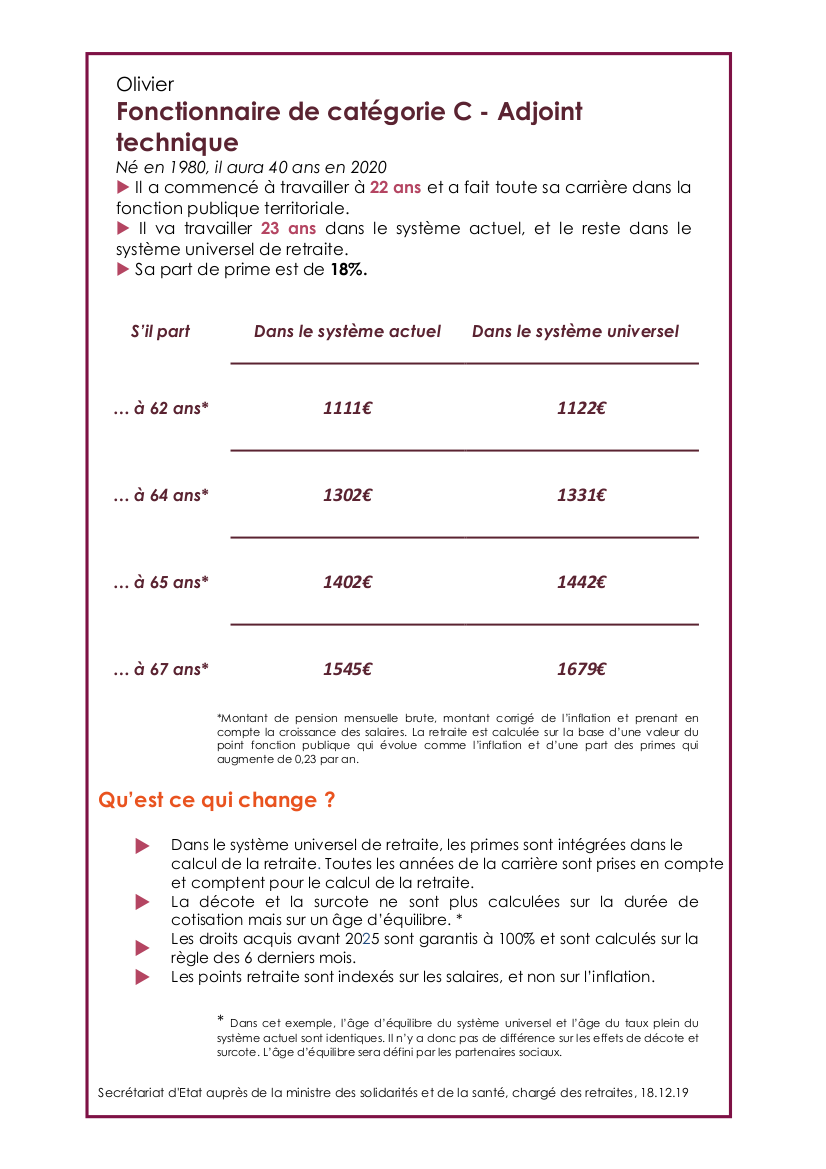
\includegraphics[height=\textheight]{g80}}
\frame{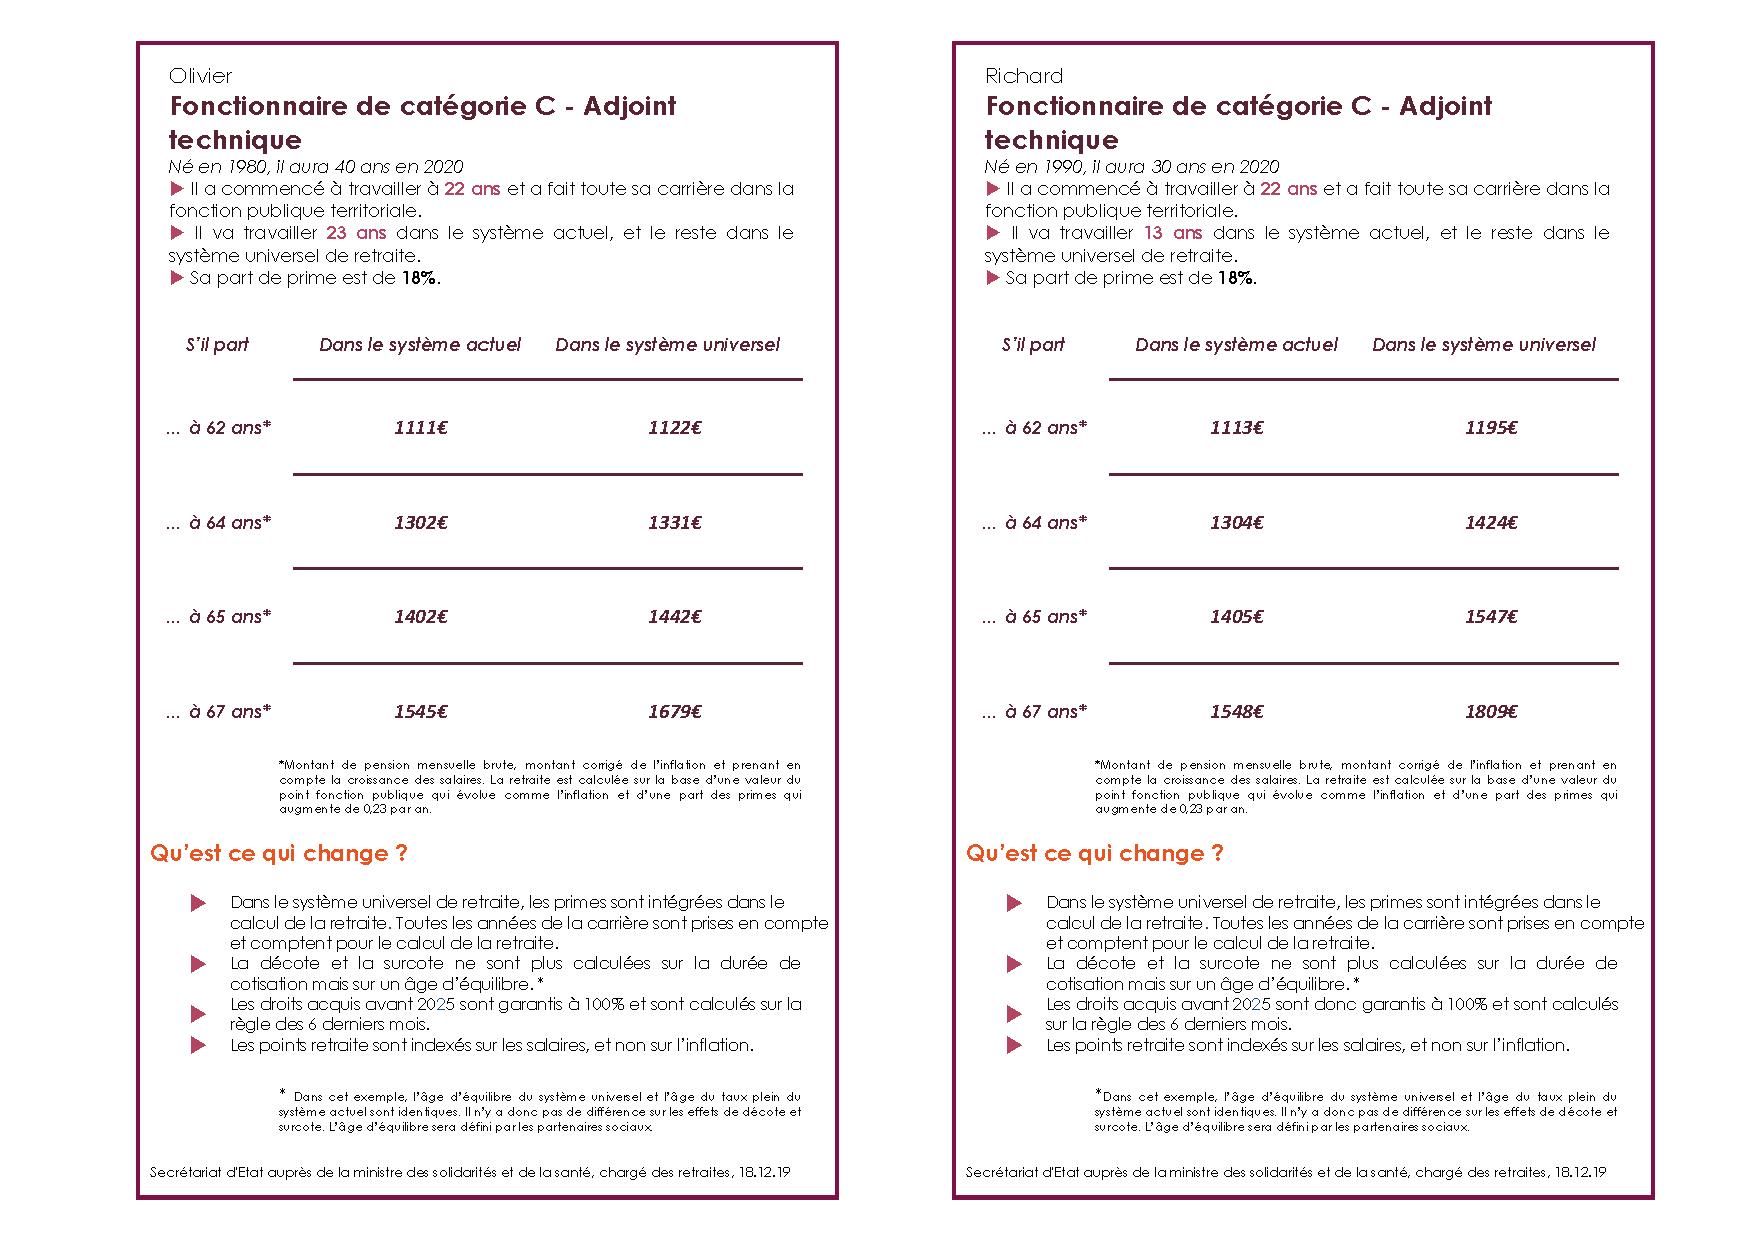
\includegraphics[width=\textwidth]{public2}}
\frame{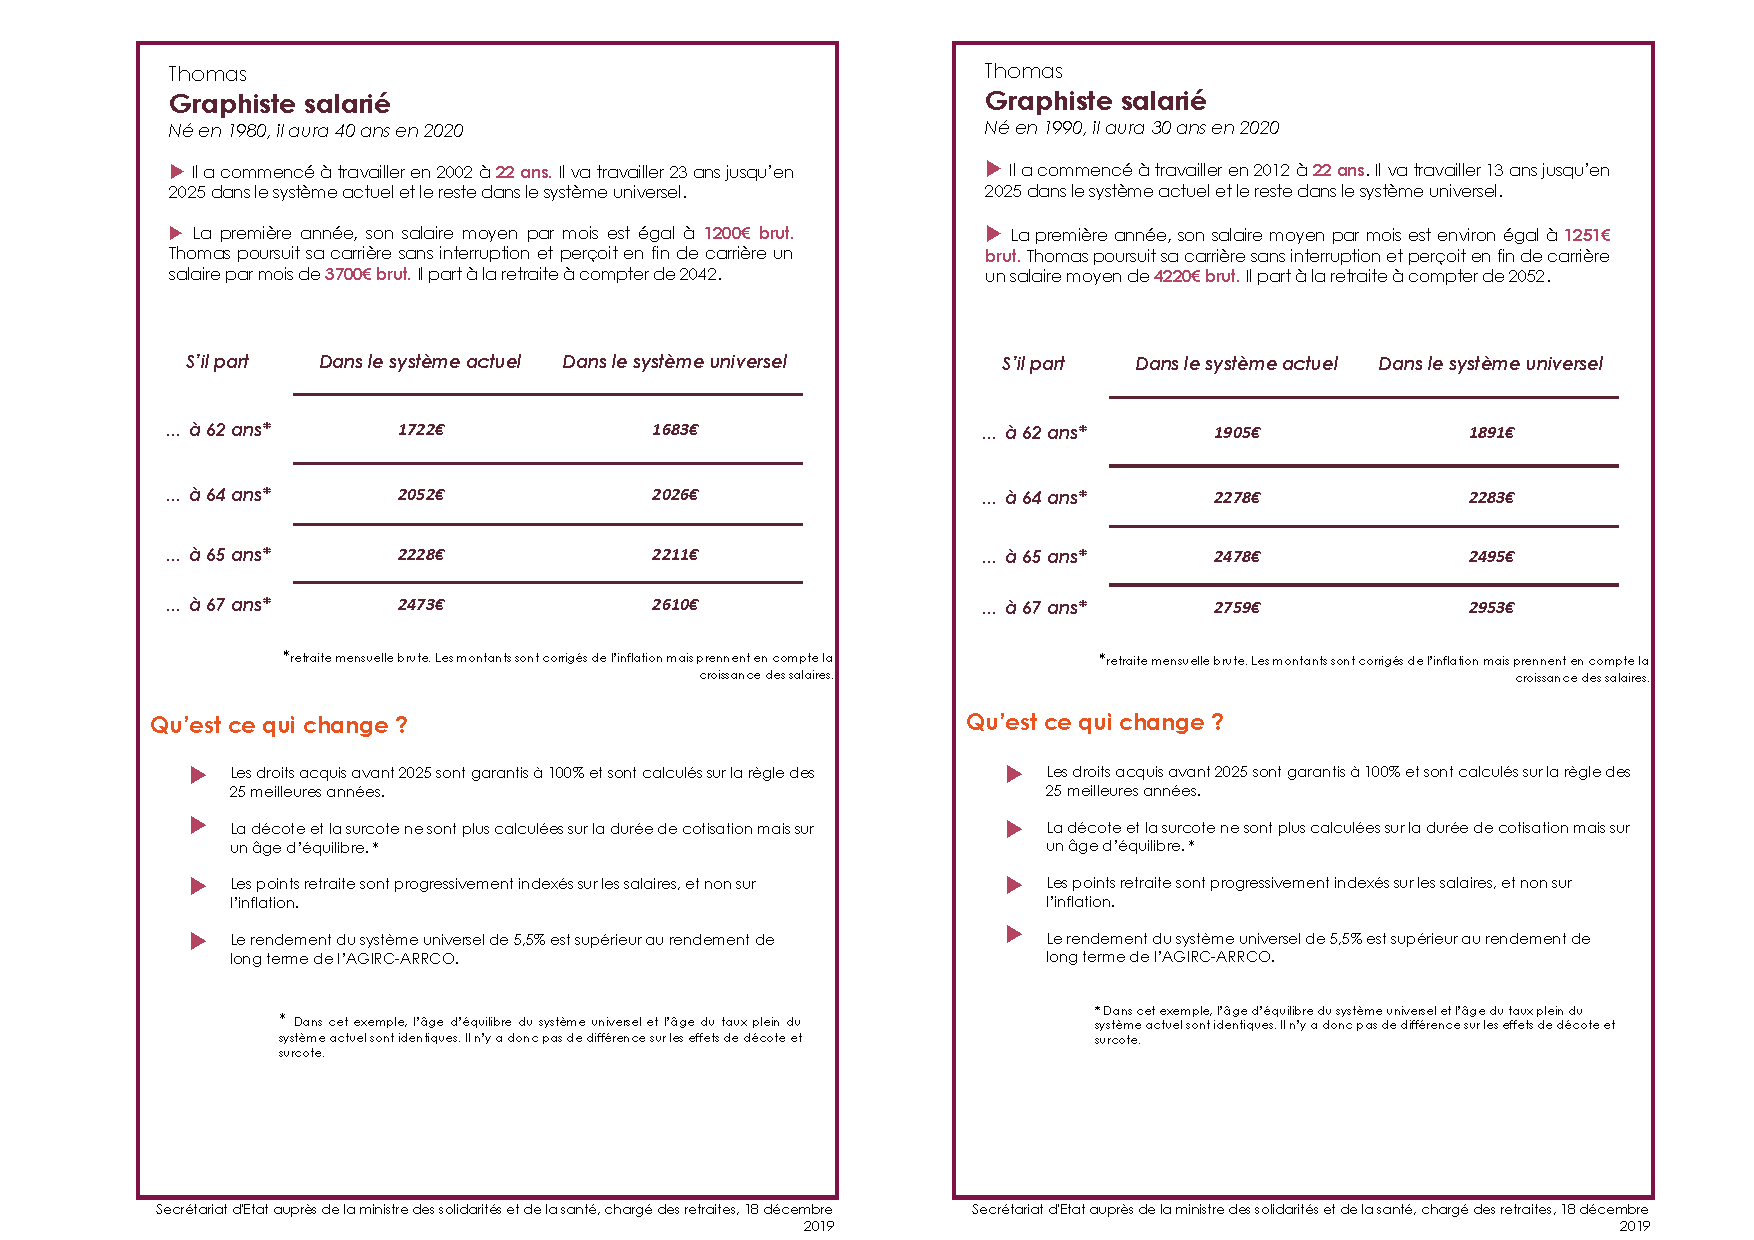
\includegraphics[width=\textwidth]{prive2}}
\frame{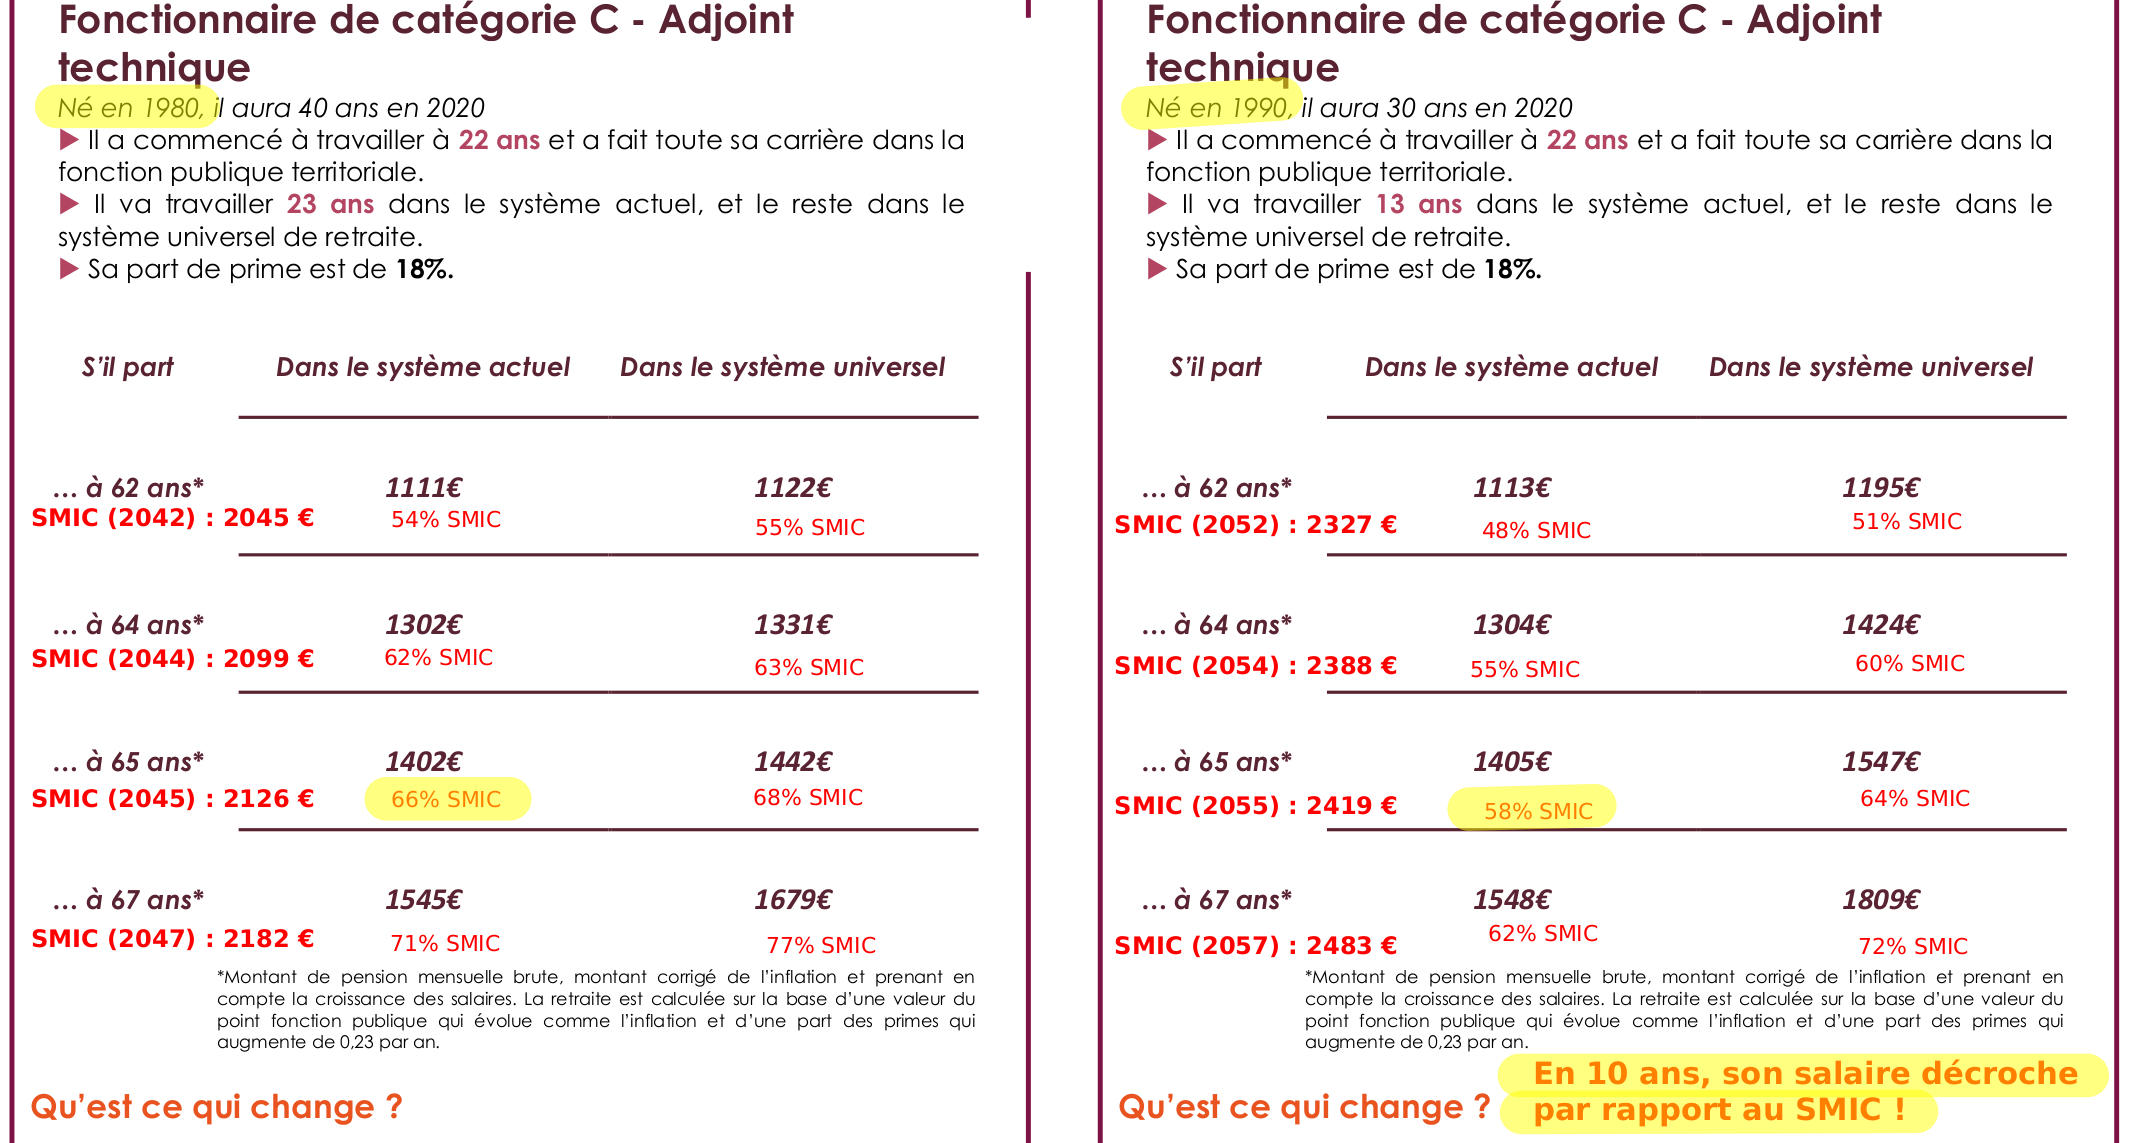
\includegraphics[width=\textwidth]{11}}

\frame{Personnel BIATSS commençant sa carrière à 22 ans en 2000:\\
  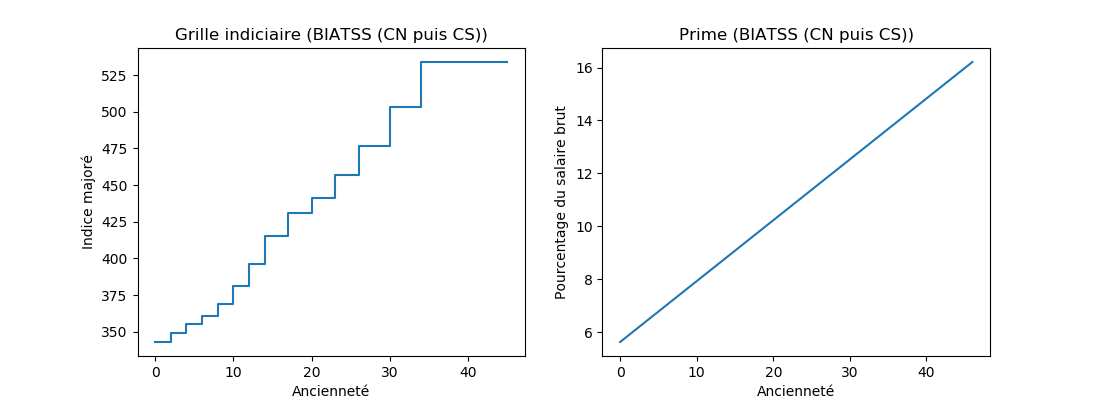
\includegraphics[width=\textwidth]{grille}\\
43 annuités en 2043, à 65 ans}

\frame{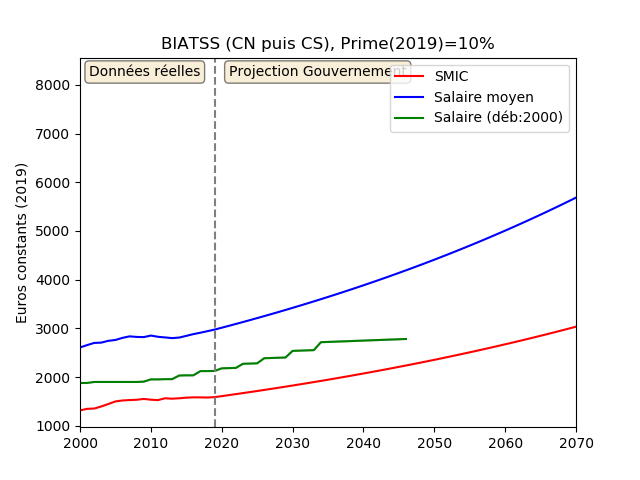
\includegraphics[width=\textwidth]{salaireEC}}

\frame{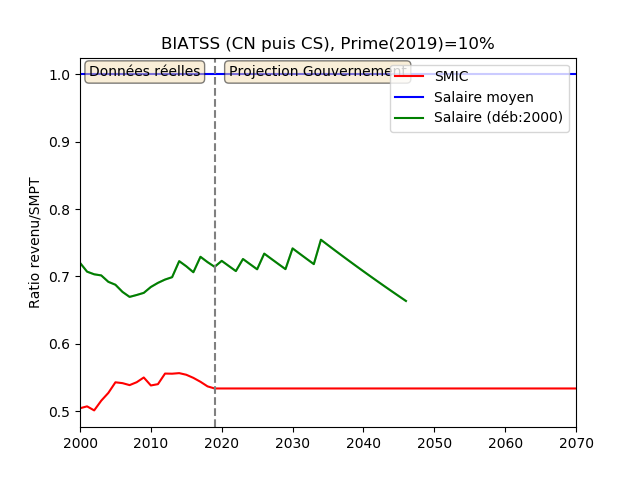
\includegraphics[width=\textwidth]{salaireRel}}



\frame{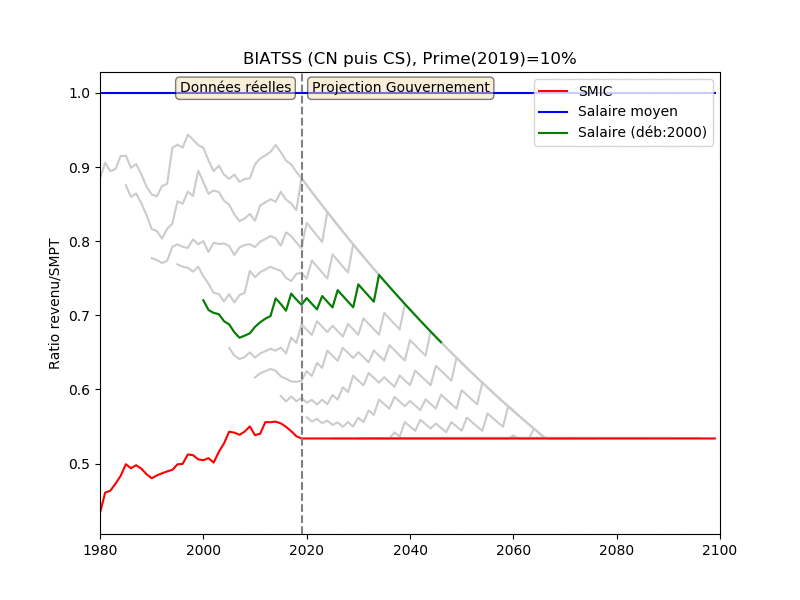
\includegraphics[width=\textwidth]{selonannee-4}}
\frame{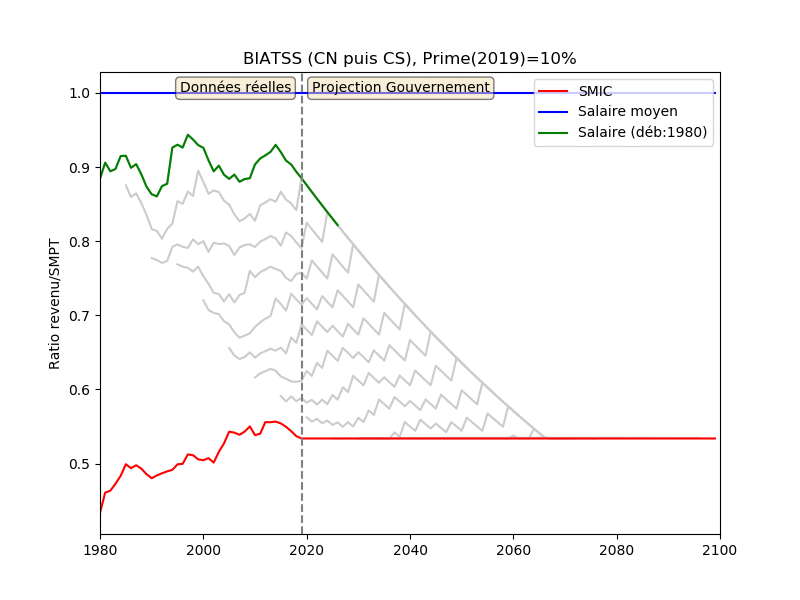
\includegraphics[width=\textwidth]{selonannee-0}}
\frame{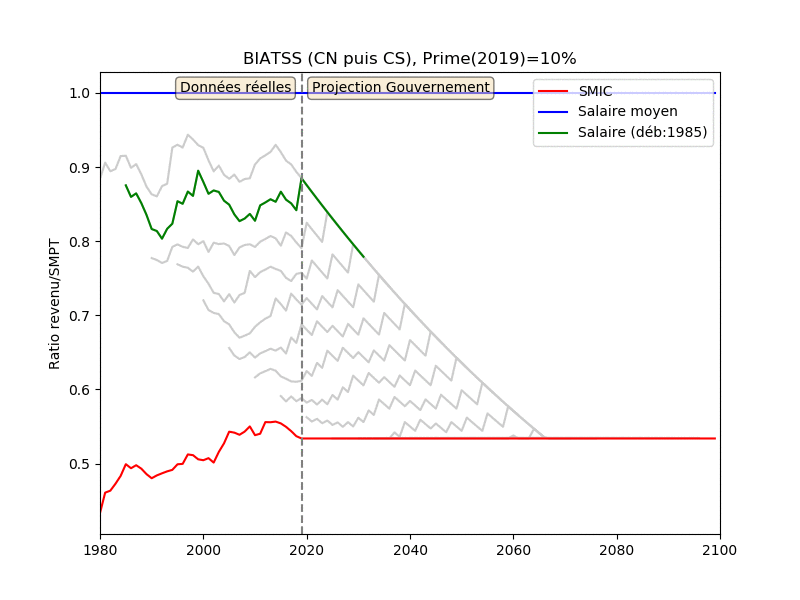
\includegraphics[width=\textwidth]{selonannee-1}}
\frame{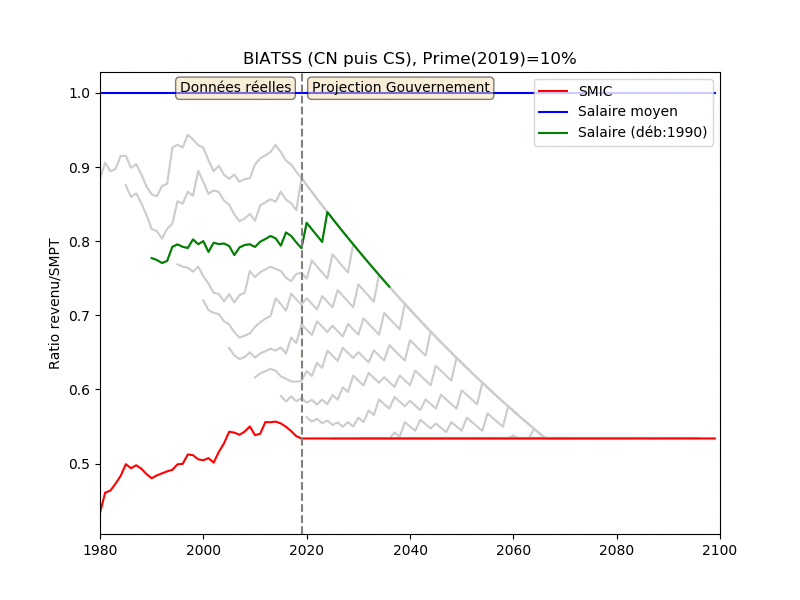
\includegraphics[width=\textwidth]{selonannee-2}}
\frame{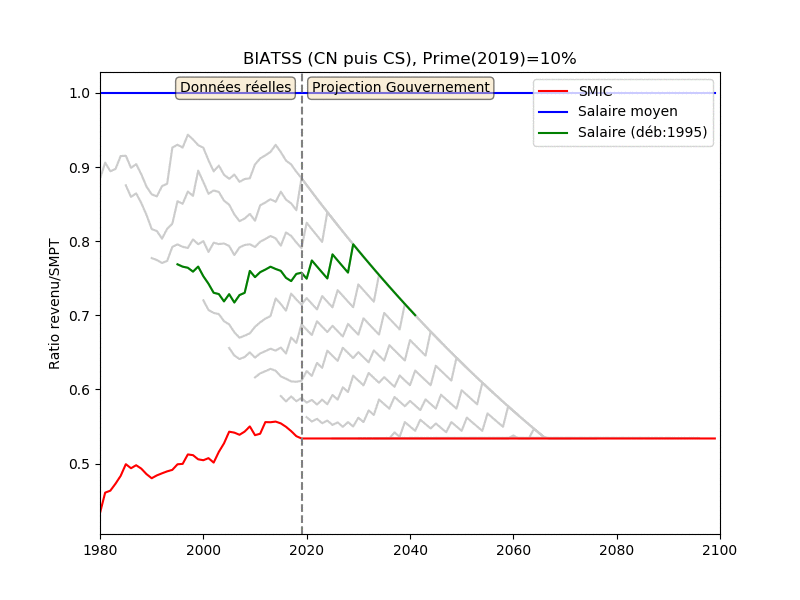
\includegraphics[width=\textwidth]{selonannee-3}}
\frame{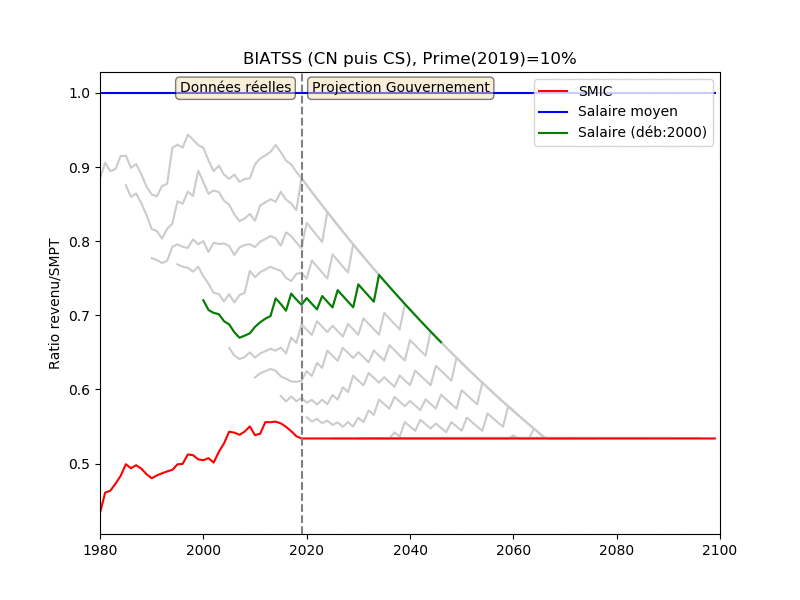
\includegraphics[width=\textwidth]{selonannee-4}}
\frame{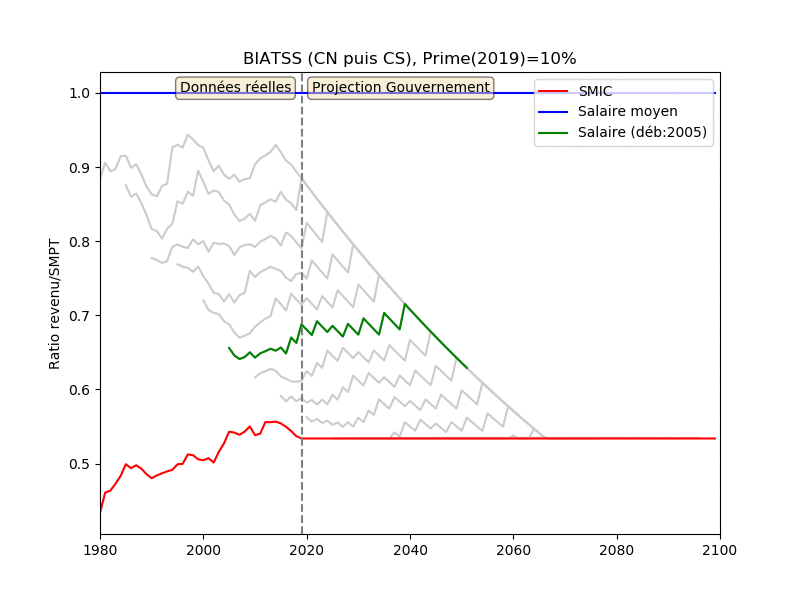
\includegraphics[width=\textwidth]{selonannee-5}}
\frame{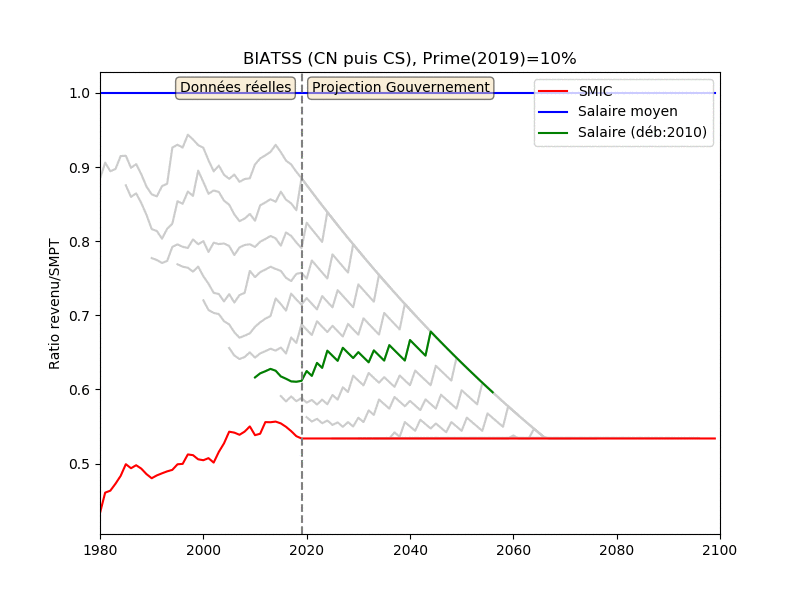
\includegraphics[width=\textwidth]{selonannee-6}}
\frame{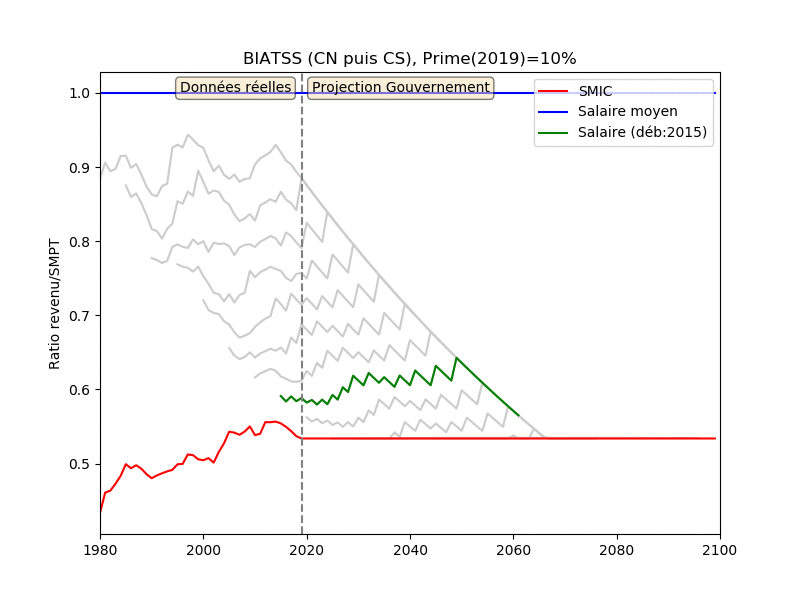
\includegraphics[width=\textwidth]{selonannee-7}}
\frame{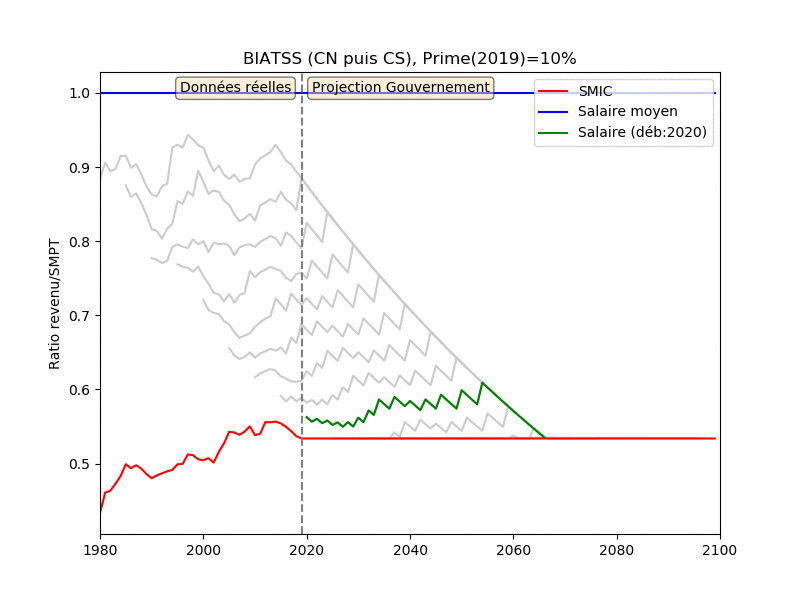
\includegraphics[width=\textwidth]{selonannee-8}}
\frame{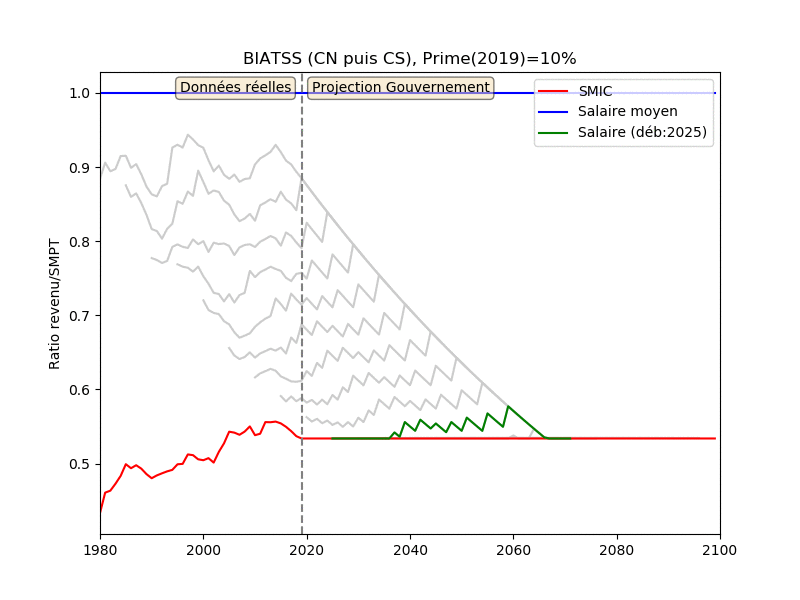
\includegraphics[width=\textwidth]{selonannee-9}}
\frame{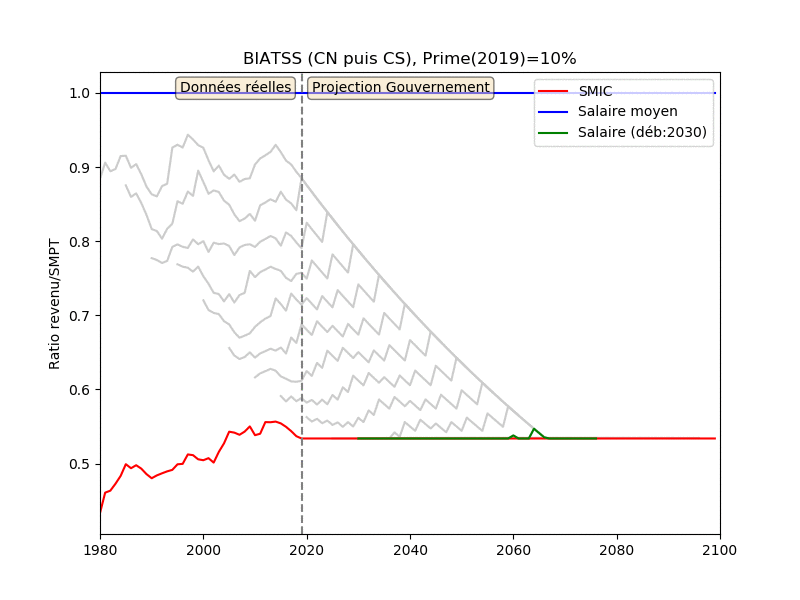
\includegraphics[width=\textwidth]{selonannee-10}}
\frame{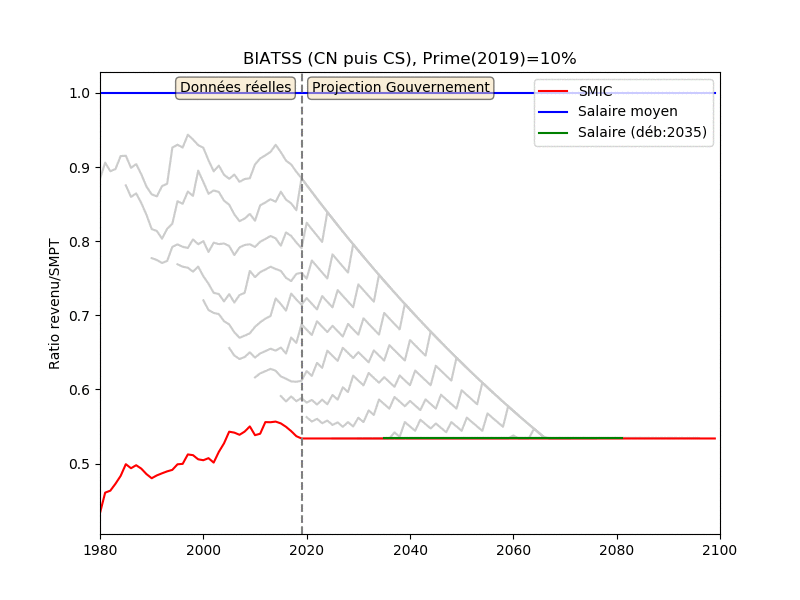
\includegraphics[width=\textwidth]{selonannee-11}}

\frame{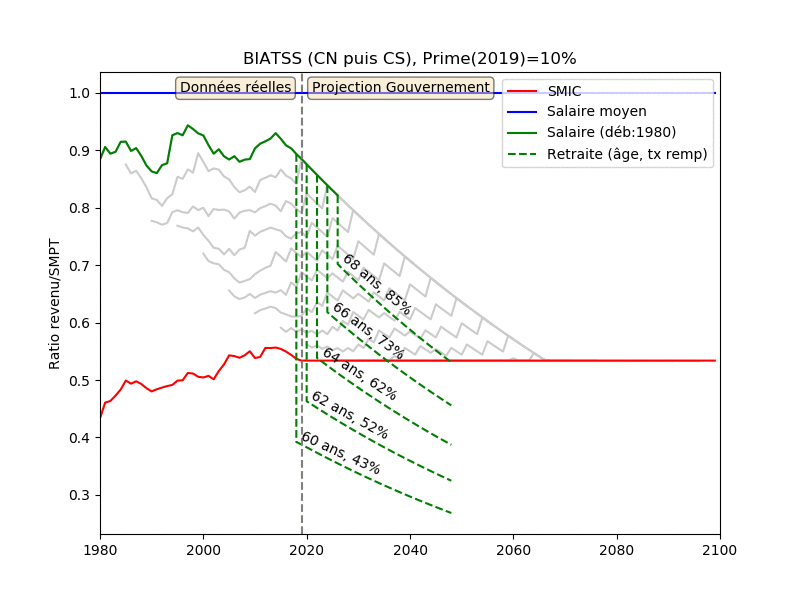
\includegraphics[width=\textwidth]{selonannee_retraite-0}}
\frame{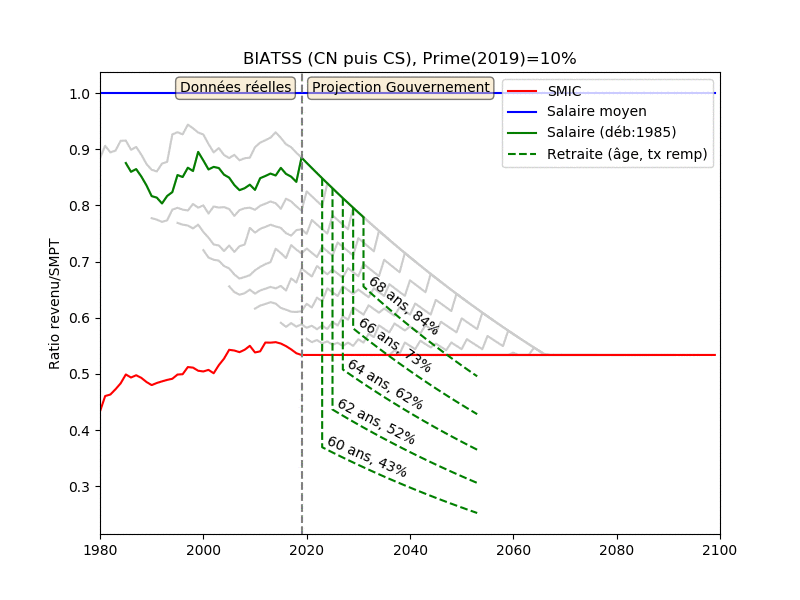
\includegraphics[width=\textwidth]{selonannee_retraite-1}}
\frame{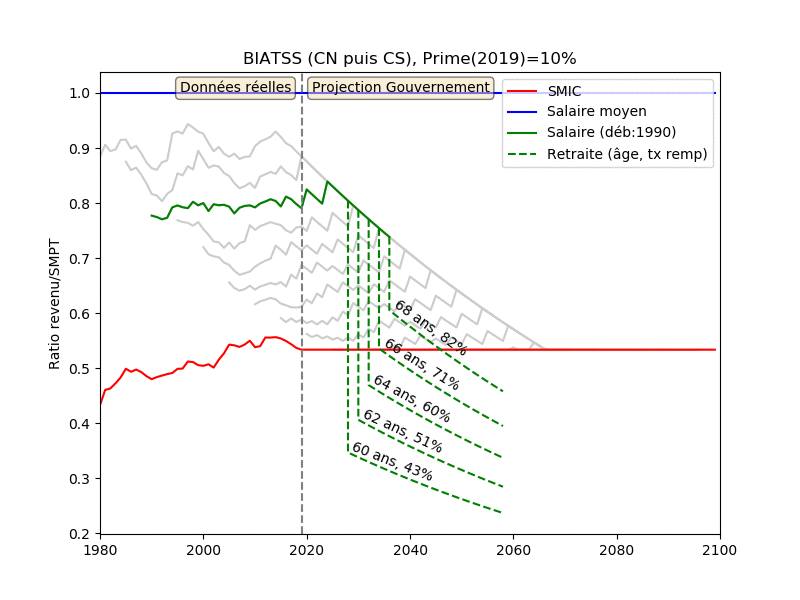
\includegraphics[width=\textwidth]{selonannee_retraite-2}}
\frame{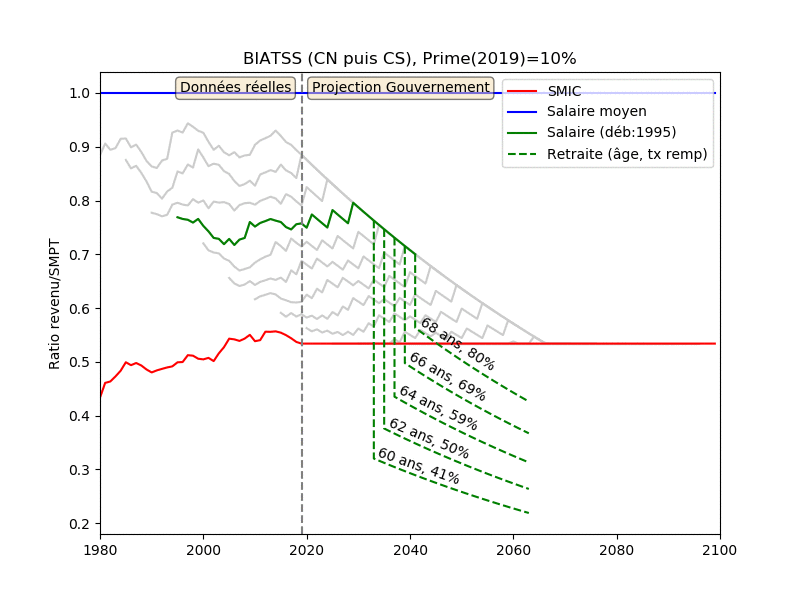
\includegraphics[width=\textwidth]{selonannee_retraite-3}}
\frame{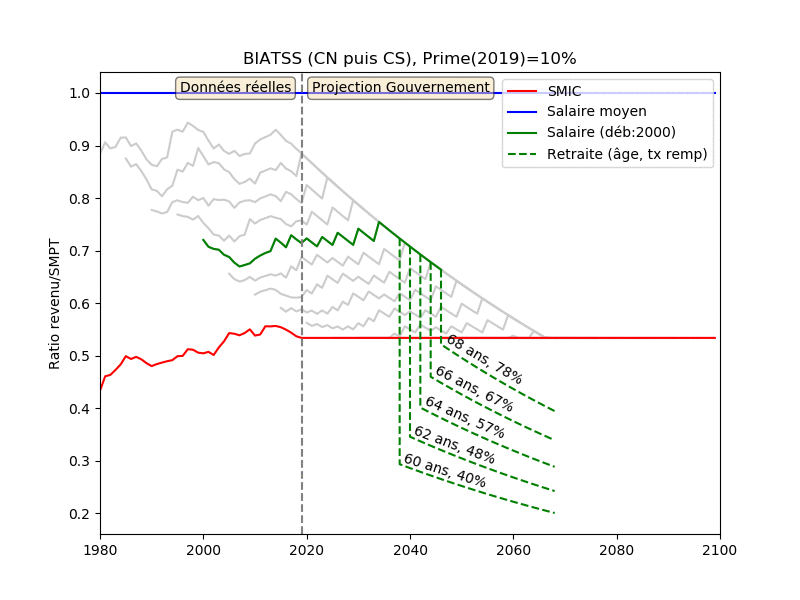
\includegraphics[width=\textwidth]{selonannee_retraite-4}}
\frame{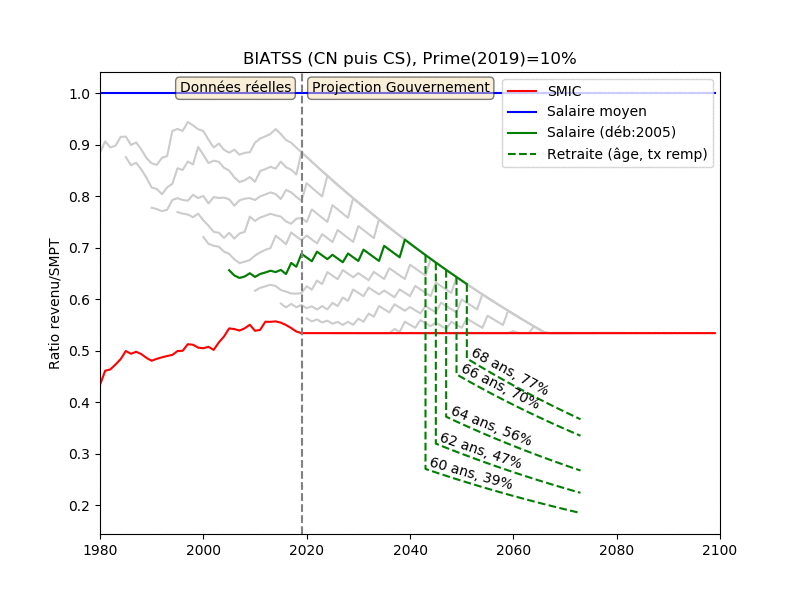
\includegraphics[width=\textwidth]{selonannee_retraite-5}}
\frame{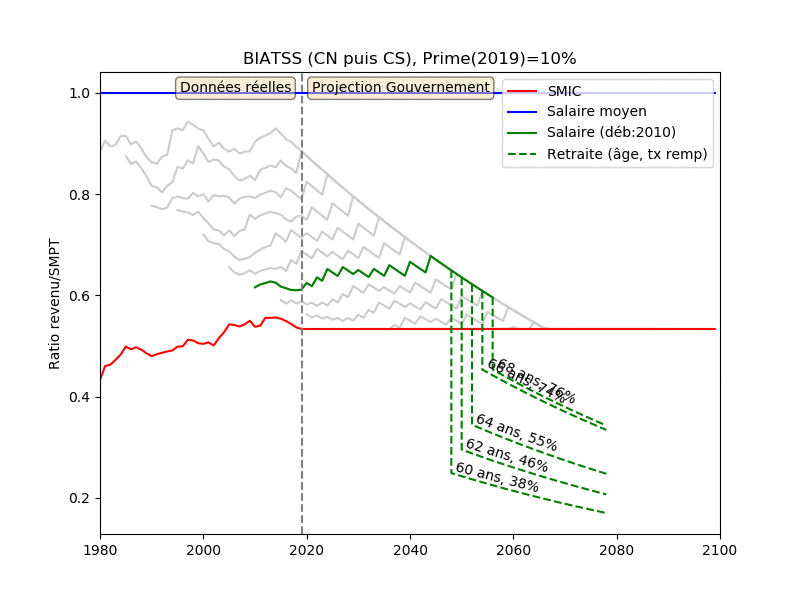
\includegraphics[width=\textwidth]{selonannee_retraite-6}}
\frame{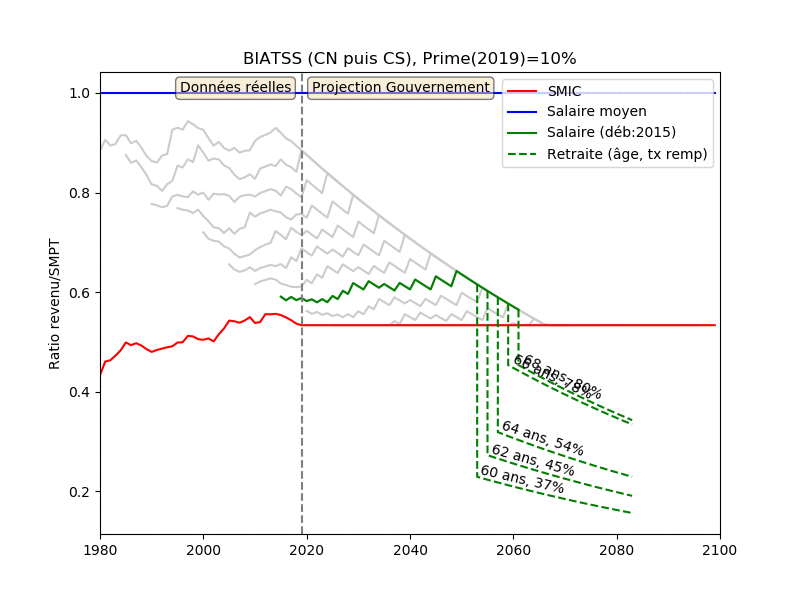
\includegraphics[width=\textwidth]{selonannee_retraite-7}}
\frame{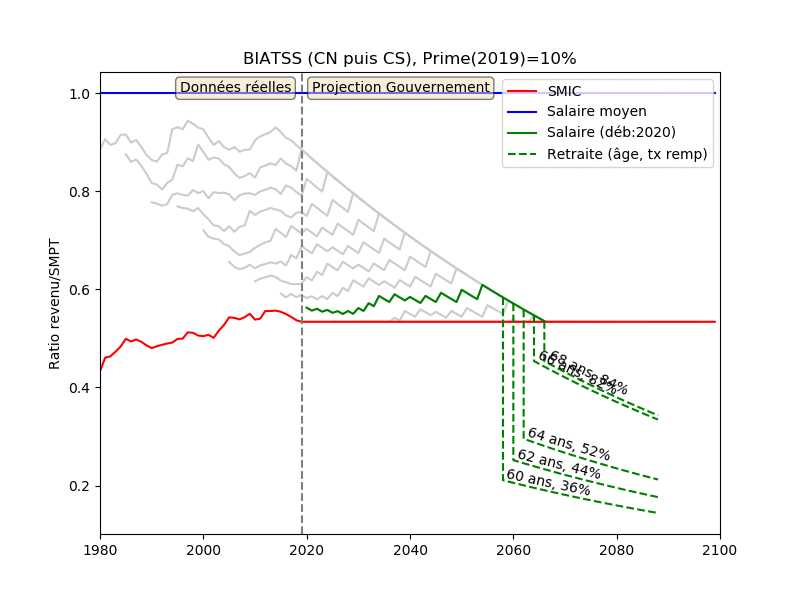
\includegraphics[width=\textwidth]{selonannee_retraite-8}}
\frame{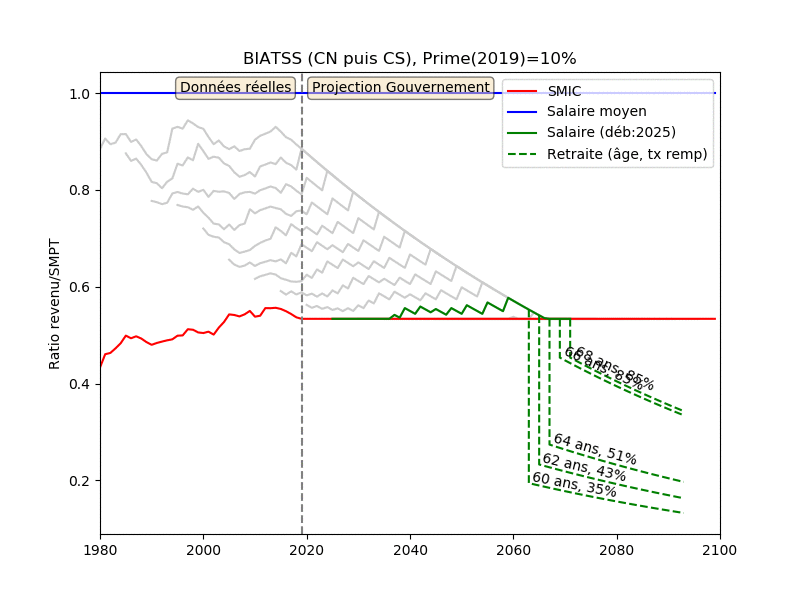
\includegraphics[width=\textwidth]{selonannee_retraite-9}}
\frame{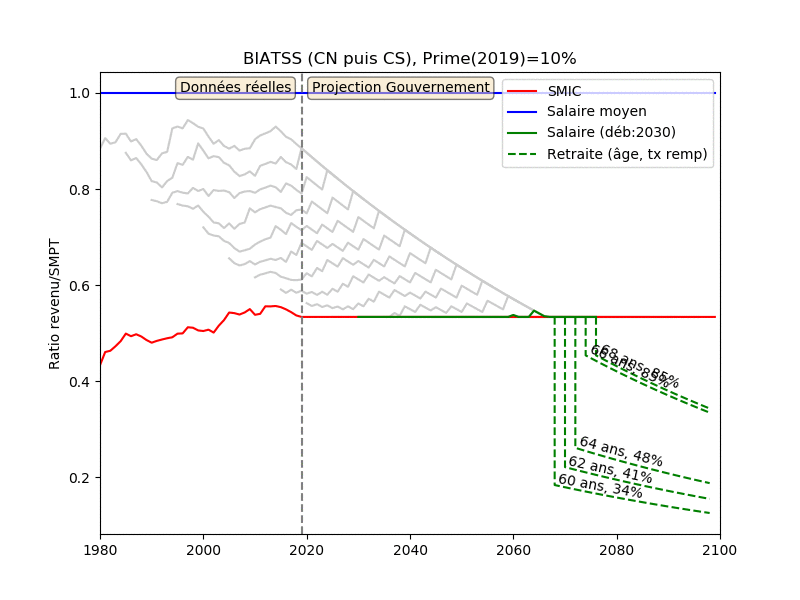
\includegraphics[width=\textwidth]{selonannee_retraite-10}}
\frame{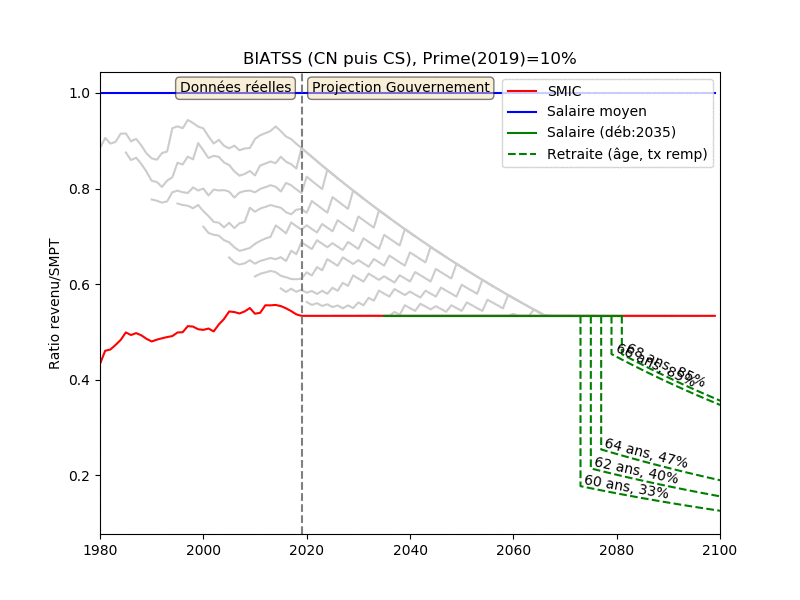
\includegraphics[width=\textwidth]{selonannee_retraite-11}}

\frame{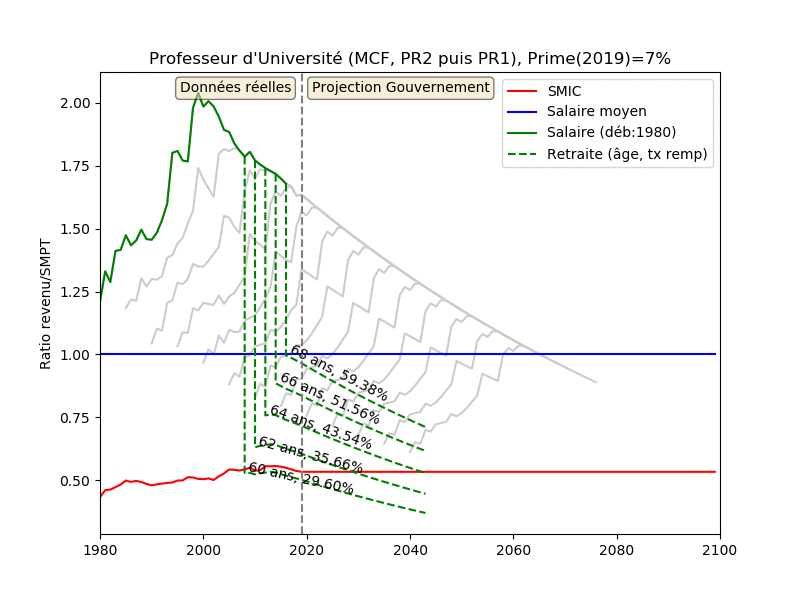
\includegraphics[width=\textwidth]{Ratio_Gouvernement_PR_7-0}}
\frame{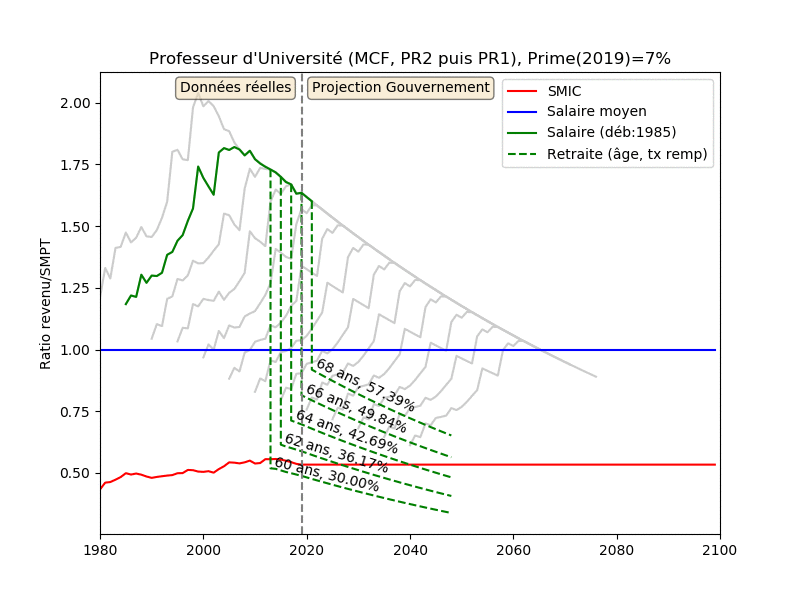
\includegraphics[width=\textwidth]{Ratio_Gouvernement_PR_7-1}}
\frame{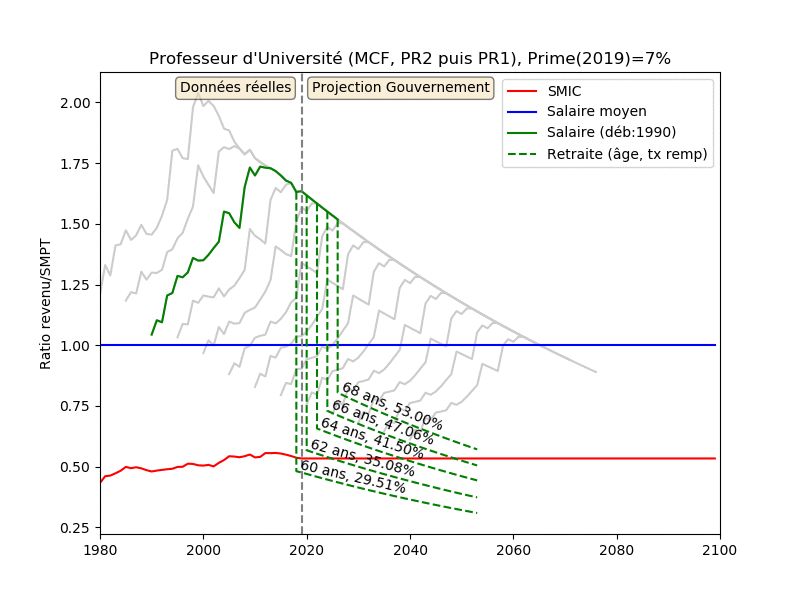
\includegraphics[width=\textwidth]{Ratio_Gouvernement_PR_7-2}}
\frame{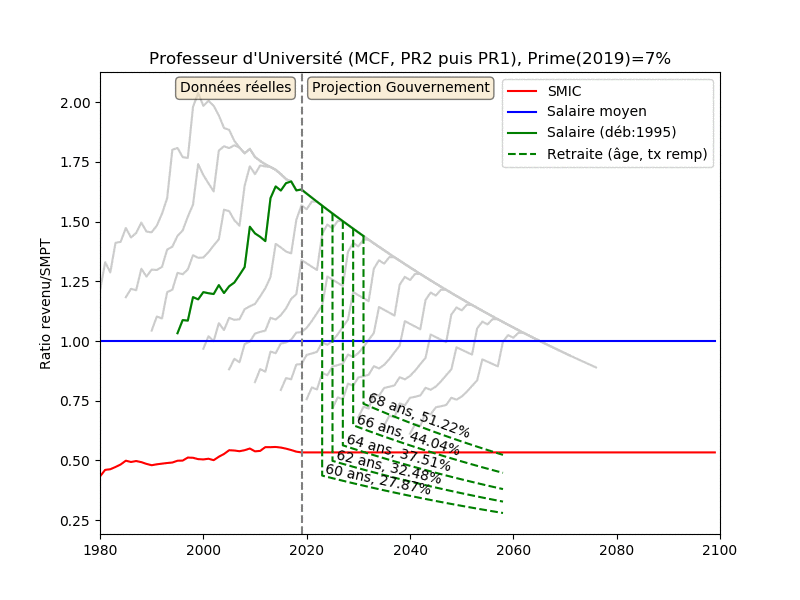
\includegraphics[width=\textwidth]{Ratio_Gouvernement_PR_7-3}}
\frame{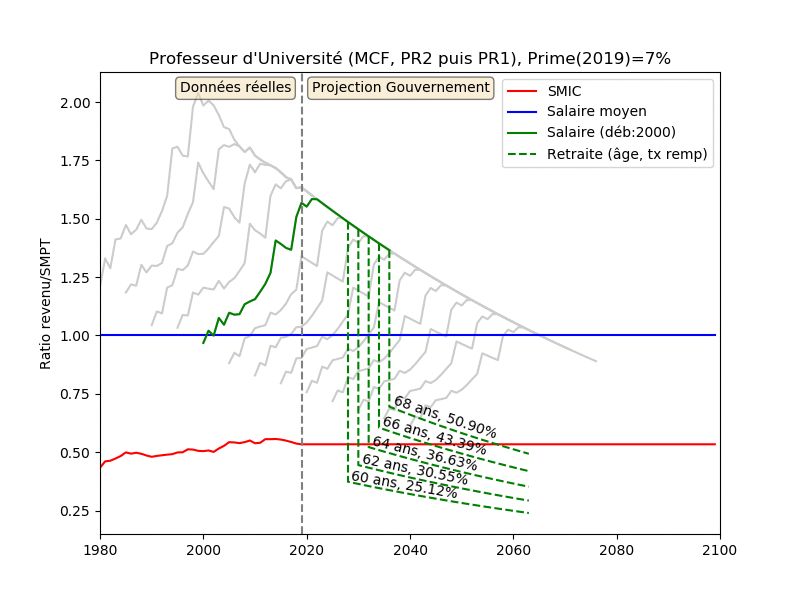
\includegraphics[width=\textwidth]{Ratio_Gouvernement_PR_7-4}}
\frame{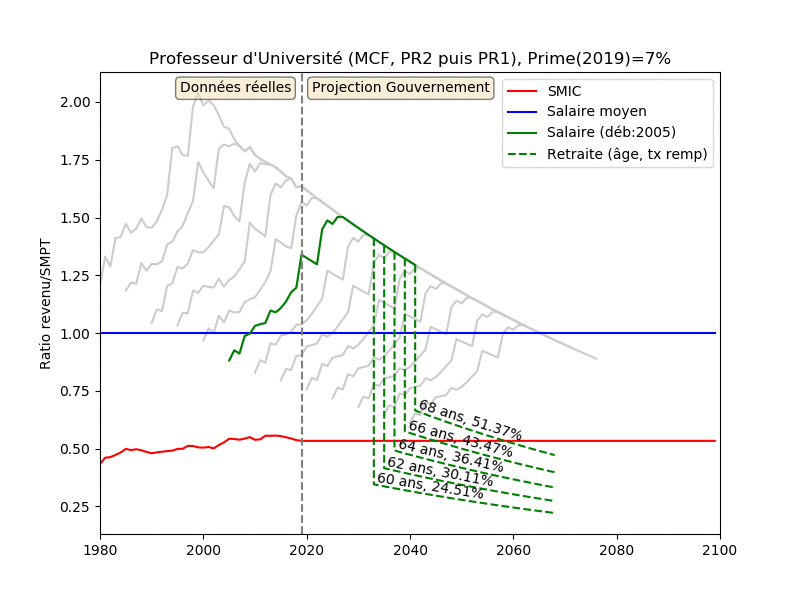
\includegraphics[width=\textwidth]{Ratio_Gouvernement_PR_7-5}}
\frame{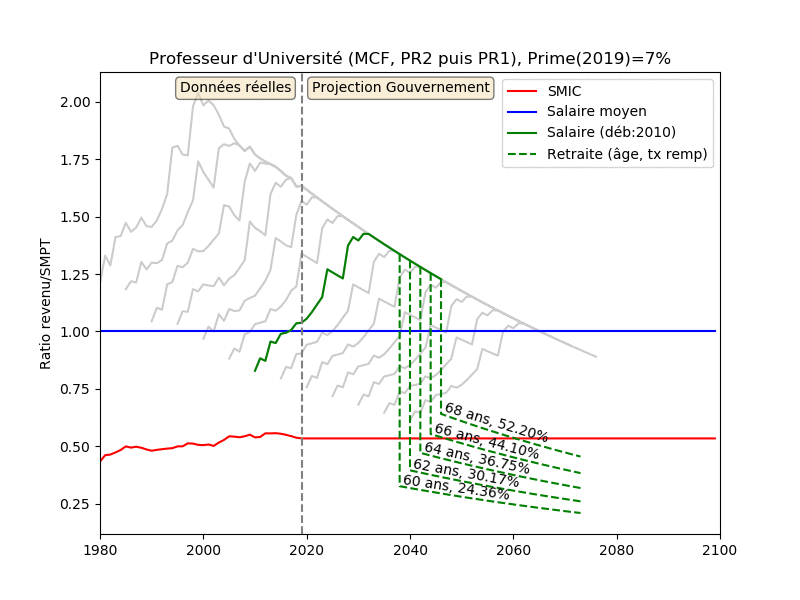
\includegraphics[width=\textwidth]{Ratio_Gouvernement_PR_7-6}}
\frame{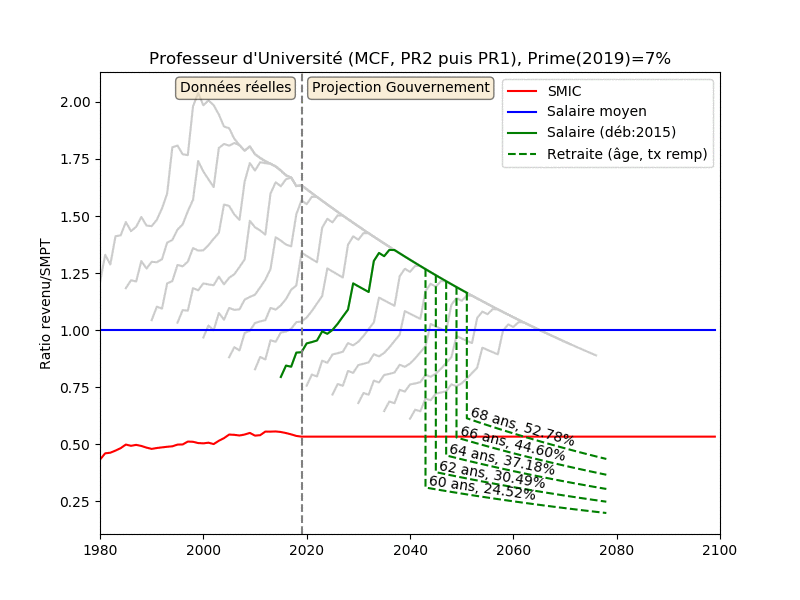
\includegraphics[width=\textwidth]{Ratio_Gouvernement_PR_7-7}}
\frame{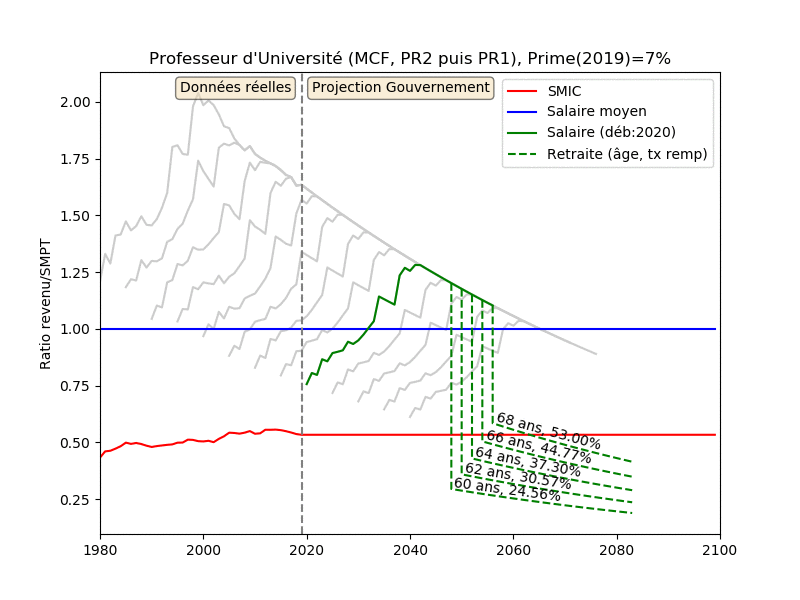
\includegraphics[width=\textwidth]{Ratio_Gouvernement_PR_7-8}}
\frame{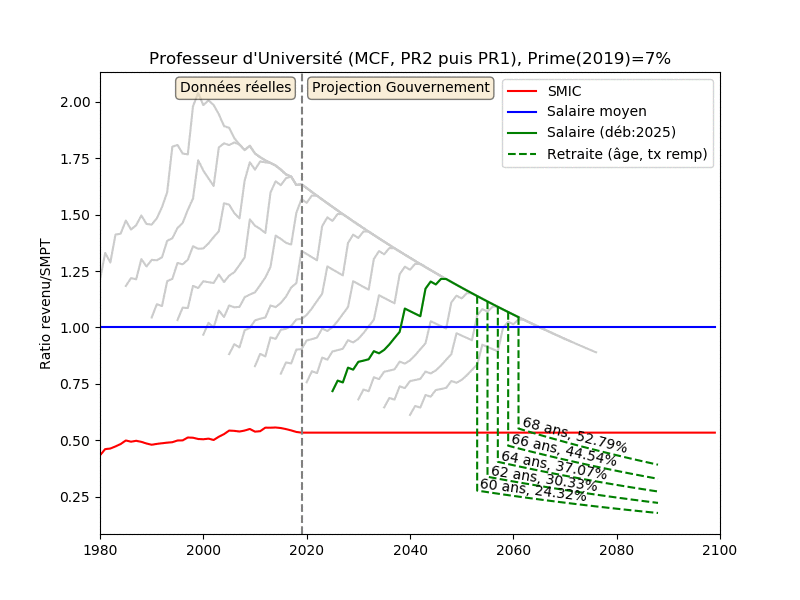
\includegraphics[width=\textwidth]{Ratio_Gouvernement_PR_7-9}}
\frame{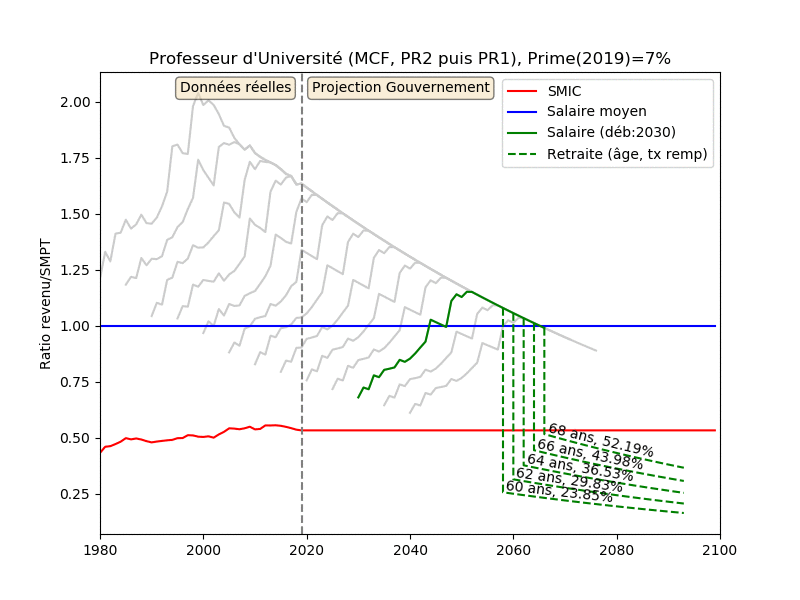
\includegraphics[width=\textwidth]{Ratio_Gouvernement_PR_7-10}}
\frame{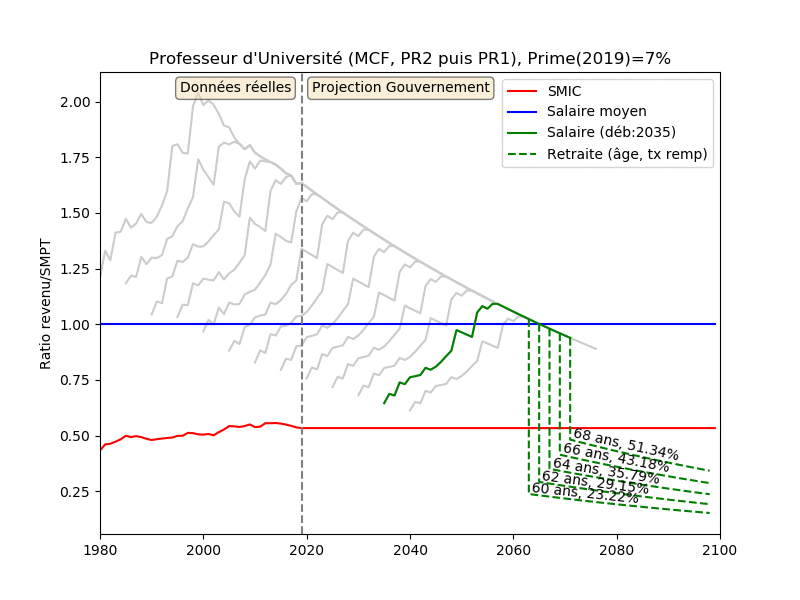
\includegraphics[width=\textwidth]{Ratio_Gouvernement_PR_7-11}}
\frame{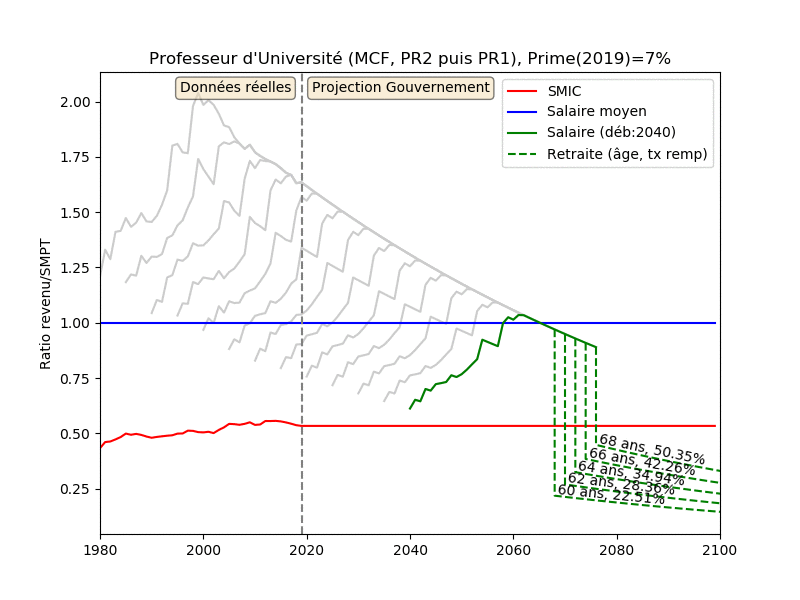
\includegraphics[width=\textwidth]{Ratio_Gouvernement_PR_7-12}}

\frame{
\frametitle{Conclusion 1}

Nous devrions nous battre pour
\begin{itemize}
\item  l'augmentation du point d'indice de la fonction publique en proportion de la croissance (du PIB)
\item la revalorisation des retraites en proportion de la croissance (du PIB)
\item le retrait du système à points (qui est d'autant plus violent que les carrières seraient revalorisées!)
\end{itemize}
}

\section{Analyse macro-économique}
\tocb

\frame{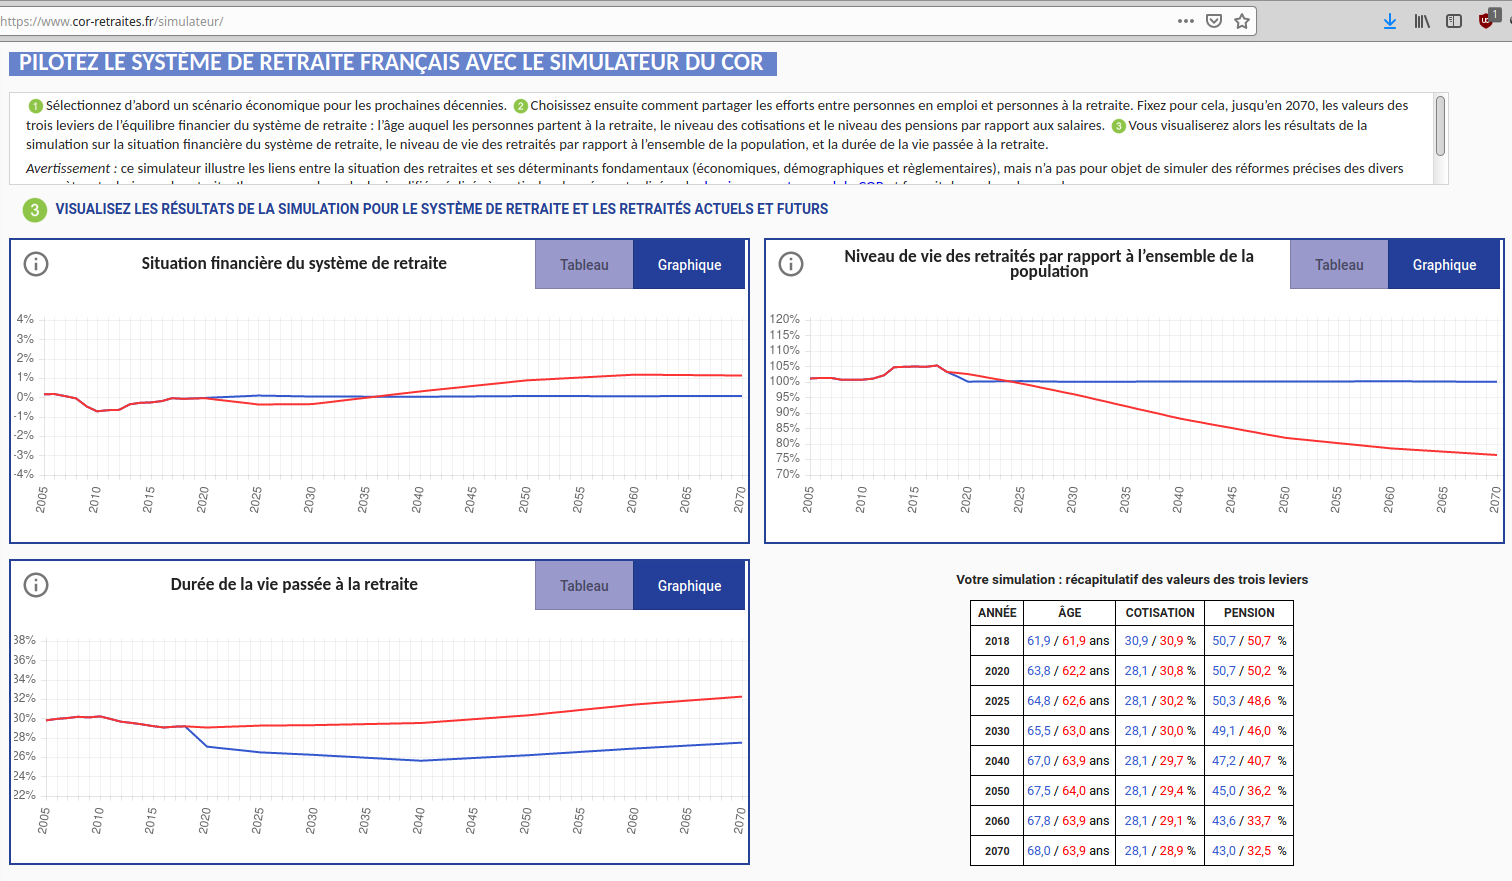
\includegraphics[width=\textwidth]{s1}}

\frame{\centering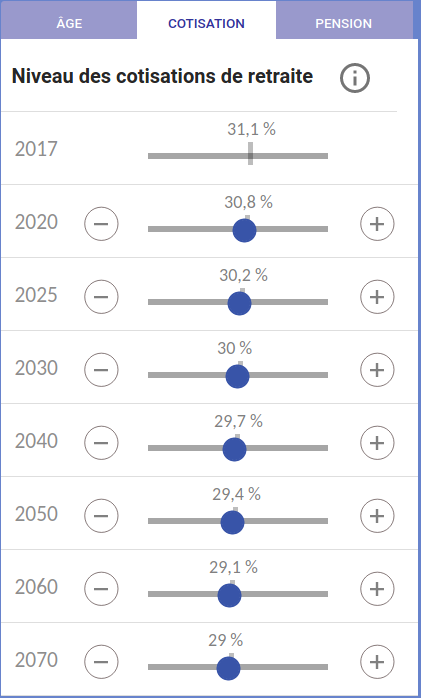
\includegraphics[height=0.9\textheight]{cortaux}}

\frame{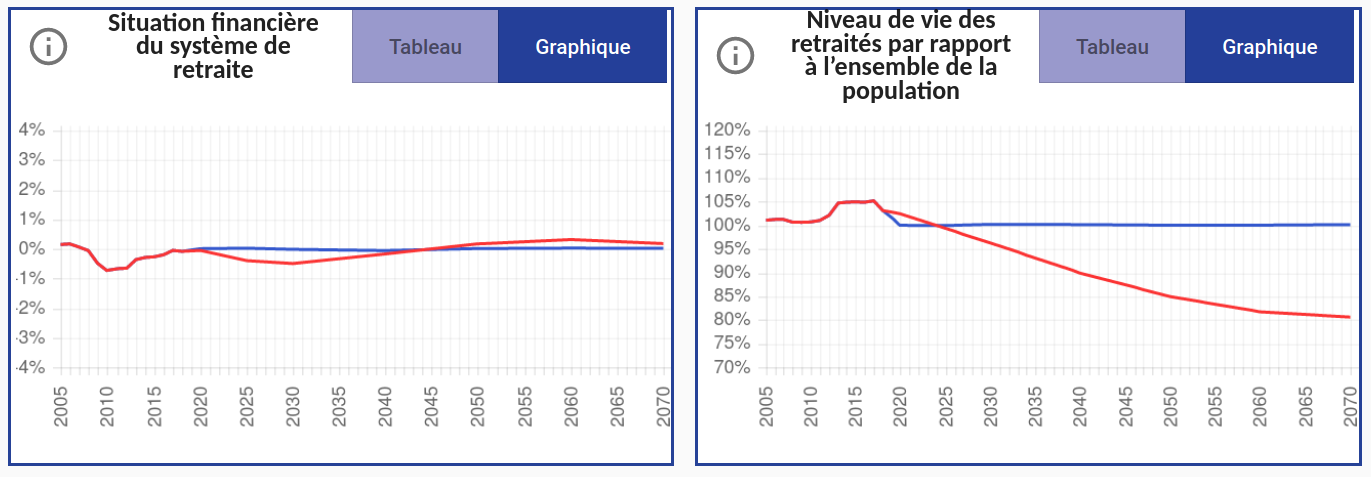
\includegraphics[width=\textwidth]{cor2}}

\frame{\centering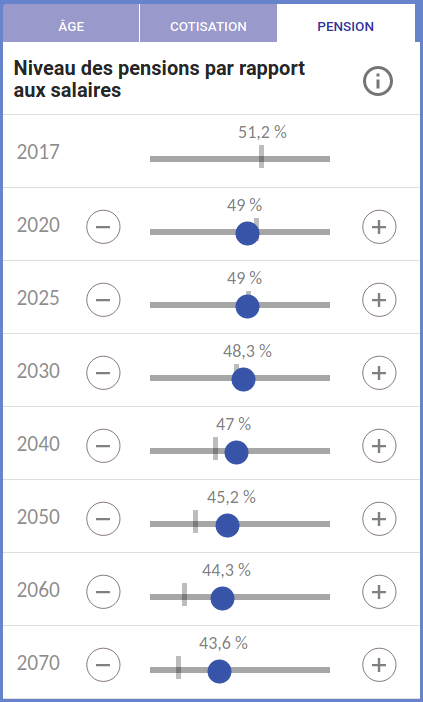
\includegraphics[height=0.9\textheight]{corpension}}

\frame{\centering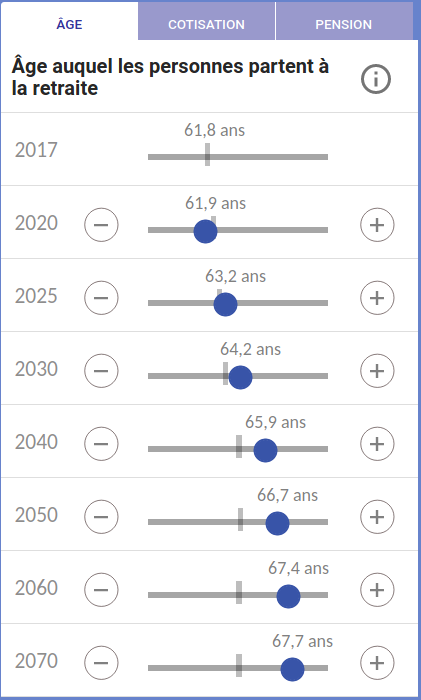
\includegraphics[height=0.9\textheight]{corage}}

\frame{\includegraphics[width=\textwidth]{macron_68_ans}}


\frame{\includegraphics[width=\textwidth]{macron_62_ans}}


\frame{\includegraphics[width=\textwidth]{toto-0}}

\frame{\includegraphics[width=\textwidth]{toto-1}}

\frame{\includegraphics[width=\textwidth]{simu_agepension}}

\frame{\includegraphics[width=\textwidth]{toto-2}}

\frame{\includegraphics[width=\textwidth]{toto-4}}


\frame{
  \frametitle{Conclusion 2}

  Nous devrions nous battre pour
  \begin{itemize}
  \item la hausse du taux de cotisation
  \item (une répartition plus juste/redistributive des pensions)
  \end{itemize}

  ~\\

  ~\\

  PS: L'étude d'impact est bidon (micro- et macro-économiquement) et régressive pour la fonction publique.
  
  }

\frame{\centering\includegraphics[height=\textheight]{jesus}}


\end{document}
